\documentclass{article} % For LaTeX2e
\usepackage{nips14submit_e,times}
\usepackage{hyperref}
\usepackage{url}

\usepackage{graphicx} % more modern
\usepackage{subfigure} 
\usepackage{amssymb}
\usepackage{amsmath}
\usepackage{amsthm}
\usepackage{natbib}

\usepackage{framed}

\usepackage{algorithm}
\usepackage{algorithmic}
\usepackage{amsmath}
\usepackage{epstopdf} 

\DeclareMathOperator*{\argmin}{arg\,min}
\usepackage{hyperref}
\usepackage{nameref}
\usepackage[]{mcode}

% For named refs (definitions)
% taken from: https://tex.stackexchange.com/questions/1230/reference-name-of-description-list-item-in-latex
\makeatletter
\let\orgdescriptionlabel\descriptionlabel
\renewcommand*{\descriptionlabel}[1]{%
 \let\orglabel\label
 \let\label\@gobble
 \phantomsection
 \edef\@currentlabel{#1}%
 %\edef\@currentlabelname{#1}%
 \let\label\orglabel
 \orgdescriptionlabel{#1}%
}

\newcommand{\specialcell}[2][c]{%
  \begin{tabular}[#1]{@{}c@{}}#2\end{tabular}}

%\documentstyle[nips14submit_09,times,art10]{article} % For LaTeX 2.09


\title{Computation Discovery}

%\icmlauthor{Wojciech Zaremba}{zaremba@cs.nyu.edu}
%\icmlauthor{Karol Kurach}{kkurach@google.com}
%\icmlauthor{Rob Fergus}{fergus@cs.nyu.edu}

% The \author macro works with any number of authors. There are two commands
% used to separate the names and addresses of multiple authors: \And and \AND.
%
% Using \And between authors leaves it to \LaTeX{} to determine where to break
% the lines. Using \AND forces a linebreak at that point. So, if \LaTeX{}
% puts 3 of 4 authors names on the first line, and the last on the second
% line, try using \AND instead of \And before the third author name.

\newcommand{\fix}{\marginpar{FIX}}
\newcommand{\new}{\marginpar{NEW}}

%\nipsfinalcopy % Uncomment for camera-ready version

\begin{document}


\maketitle

\begin{abstract} We present an approach based on attribute grammars
  for automatically discovering efficient ways to compute polynomial
  expressions. Our method can be regarded as
  a graph search algorithm in the space of computations, where we seek
  branches in the graph that compute the {\em exact} same expression as
  the original, but have a lower complexity. Amongst other things, it can be used
  to find a closed form expression for marginalizations involving
  polynomials. We demonstrate this on two problems which involve an
  summation over an exponential number of polynomial terms: (i) a
  Taylor-series approximation to the partition function of a binary
  RBM and (ii) a closed-form solution Dropout. 
 \end{abstract} 

\section{Introduction} \label{introduction} 

We show how the task of finding equivalent
mathematical expressions can be automated. Our focus is on finding equivalent
mathematical formulas (i.e.~which give an identical numerical result
to the original expression) for marginalization over huge sets. 
Problems involving marginalization are prevalent in machine learning, and 
exact marginalizations can be a replacement for sampling methods.

We propose a deterministic, grammar-based framework which discovers
relations between multi-variable polynomial expressions. First, we
construct an attribute grammar -- a context-free grammar extended to
contain set of attributes, introduced by Donald Knuth
\cite{knuth1968semantics}. To define the search space we use a set of
context-free grammar rules representing admissible operations. 



\begin{minipage}{\linewidth}
\begin{framed}
\begin{flushleft}
Figure 1: A toy example
\vspace{3mm}

We are given matrices $A \in \mathbb{R}^{n \times m}$, $B \in \mathbb{R}^{m \times k}$. We wish
 to compute \texttt{sum(sum(A*B))}, i.e.~: 
\vspace{1.5mm} \\ 
$\sum_{n,k} AB = \sum_{i = 1}^n \sum_{j = 1}^m \sum_{l = 1}^k A_{i, j} B_{j, l} $
\vspace{1.5mm} \\ 
which naively takes $O(nmk)$ time. Our framework is able to discover
an efficient version of the formula, that computes the same result in $O(n(k+m))$
time: \texttt{sum(sum(A .* repmat(sum(B, 2), [1, n])'))}
 \vspace{1mm} \\ 
Our framework has two  distinct stages:
 \vspace{-2mm} 
 \begin{enumerate}
\item The {\em grammar tree} is built (see Algorithm 1). This contains
  an exhaustive set of all valid compositions of expressions from the
  grammar. While slow, this only needs to be performed once for a
  given grammar, irrespective of the number of target expressions we
  wish to compute. The figure below shows two branches of the grammar
  tree.
\item The framework then looks for a linear combination of tree leaves 
  to match the target expression (which requires solving a linear system).
  It chooses leafs with smallest computational complexity 
  (see Section \ref{sec:linear}). The two leaves \texttt{L$_1$} and
  \texttt{L$_2$} shown in the tree produce the same result as the target
  expression, but the latter is preffered as it has a lower complexity. 
\end{enumerate}

Empirical tests indicate that our expression is indeed faster to
compute than the naive one (see Figure \ref{ab}).

\includegraphics[scale=0.4]{img/toy_tree.pdf}
\vspace{-5mm}
\end{flushleft}
\end{framed}
%\caption{Presents how framework works to compute fast expression sum(sum(A*B)).}
\label{fig:example_ab}

\end{minipage}


\noindent
By representing the cost of every operation as a synthesized attribute
(i.e.~computed bottom-up from child node attributes) we can search for
formula with low time complexity. Through a linear combination of
grammar elements, we can find a solution to the desired
expressions. 



Figure \ref{fig:example_ab} shows our framework applied to a simple matrix expression:
\texttt{sum(sum(A*B))}, where \texttt{A} and \texttt{B} are matrices. Naively, this takes $O(n^3)$ to compute due to
the matrix multiply operation. The example outlines how our framework
can find an alternate way of computing {\em exactly} the same result,
but in $O(n^2)$ time. We start with this simple (non-machine learning example) to
explain how system works.

We demonstrate the flexibility of our technique by applying it to 
various problems in machine learning: 
\begin{enumerate}
\vspace{-2mm}
\item Approximation of the partition function of a binary RBM using a
  Taylor series. We can produce an exact 6th order 
  approximation which is
  computable in closed-form, and takes polynomial time.
  Naive evaluation of the Taylor-series
  approximation would require summing over the $2^n$ possible states.   
\item Closed-form computation of Dropout for rational activation functions. 
  Dropout \cite{hinton2012improving}
  involves the  stochastic deletion of outputs within a dense neural
  network layer at training time. For $n$ output units, the $2^n$
  possible deletion patterns are sampled independently for each
  training sample. We use our framework to derive a closed-form
  expression that integrates out over all $2^n$ states (Section \ref{sec:dropout}).
% \item Data augmentation is for object recognition purposes it consists
%   translations, rotations, contrast alternation and few others. 
%   We how to construct update rule to weights which
%   integrates over all data jitterings, and contrast alternations (Section \ref{sec:augm}).
\end{enumerate}
\vspace{-2mm}

The main contribution of the paper is the introduction of a general
framework for discovering efficient closed-form expressions. This are
of the main use for marginalization problems (or sum over large number of
expressions). Its
flexibility means can be used on a wide range of problems encountered
in math and AI, beyond those outlined above. We dedicate follow up 
papers to address properly each of aforementioned applications. This
paper focuses mainly on framework description, and gives only brief description
of applications. By the time of publication, we will release Matlab and python
code to generate computations described in this paper.


\section{Related Work} \label{relatedwork}

The attribute grammar, originally developed in 1968 by Knuth \cite{knuth1968semantics} in context of compiler
construction, has been successfully used as a tool for design, formal specification
and implementation of practical systems. It has influenced areas of
Computer Science such as natural language processing \cite{hafiz2011modular}, \cite{starkie2002inferring}, 
definite clause grammars \cite{bratko2001prolog}, query processing \cite{koch2007attribute}, \cite{ramakrishnan1991top} and specification of algorithms \cite{bellanova1984examples}.
Thirunarayan \cite{thirunarayan2009attribute} provides a good overview of 
applications, including static analysis of programs, program translation, specifying information
extraction algorithms and optimization of datalog programs.

In our work, we apply attribute grammars to an optimization problem. This has previously been explored in range of domains: from well-known algorithmic problems 
like knapsack packing \cite{o2004solving}, through bioinformatics \cite{waldispuhl2002approximate} to music domain\cite{desainte1994using}.
However, we are not aware of any previous work related to discovering mathematical formulas. The closest work to ours can be found in \cite{cheung1999attribute} which involves searching
over the space of algorithms and the grammar attributes are also computational complexity.




\section{Terminology}
We define the following vocabulary: 

\begin{description}
  \item[Space of matrices of polynomials\label{itm:spacematrices}] \hfill \\ A matrix of homogeneous polynomials, which we denote by $\mathcal{P}^{n \times m}_{\alpha}$. Upper index indicates size of matrix, and lower indicates degree. For instance, $\begin{pmatrix} a^3 + b^3 & b^3 + bc^2 + c^3\\ cd^2 & d^3 \end{pmatrix} \in \mathcal{P}^{2 \times 2}_3$. 

\item[Grammar\label{itm:grammar}] \hfill \\ An attributive grammar, with \ref{itm:production} defined on \ref{itm:expression}s and semantic rules on \ref{itm:attribute}s. The attributes associated to every \ref{itm:expression}, are: \ref{itm:computation}, \ref{itm:time} and \ref{itm:term}.

\item[Production rules\label{itm:production}] \hfill \\ Syntactic rules defined on \ref{itm:expression}s (transformation \ref{itm:expression} $\rightarrow$ \ref{itm:expression}), with associated semantic rules on \ref{itm:attribute}s. They are defined in figures \ref{rulestwo} and \ref{rules}. (TODO: why figure ref doesn't work?)

\item[Expression\label{itm:expression}] \hfill \\ Matrices of polynomials having a homogeneous degree $\alpha$. They belong to the spaces $\mathcal{P}^{n \times m}_\alpha$. Different expressions might be in different spaces, and it restricts which production rules can be applied. Every expression has associated \ref{itm:attribute}s

\item[Attribute\label{itm:attribute}] \hfill \\
  A value associated with \ref{itm:expression}. 

\item[Computation\label{itm:computation}] \hfill \\ A piece of code to compute given \ref{itm:production} on particular architecture or programming language. In our rules we consider Matlab as
  underlaying computation language. For example, in Matlab the transpose
  operation on matrix $\mathbb{A}$ is denoted as $\mathbb{A}'$, so our computation
  for transpose production is $\mathbb{A}'$. If we ever decide to implement our framework in R,
  the Computation for transpose would be $t(\mathbb{A})$. Computation is an \ref{itm:attribute}.

\item[Time\label{itm:time}] \hfill \\ A computation time for a particular architecture and programming language (seconds), or computation complexity (polynomial). It is an \ref{itm:attribute}.

\item[Term\label{itm:term}] \hfill \\ An instance of \ref{itm:expression}. It is an \ref{itm:attribute}.

%Let's consider a literal $L = (\mathbb{E}, \mathcal{C}, t_\mathcal{C})$. $\mathbb{E}$ is a polynomial in $\mathcal{P}^{n \times m}_{\alpha}$. $\mathcal{C}$ is a computation of this polynomial starting with a input matrices. Result of computation is a real matrix
%in $\mathbb{R}^{n \times m}_k$, which is computed in time $t_\mathcal{C}$. This time is a time necessary to perform computation on instantiations of matrices with actual values -- not computation during grammar derivation, which would involve expressions. For example, if $\mathcal{C}$ is an elementwise multiplication operation (see rules in \ref{rules}) then $t_\mathcal{C}$ would be $O(nm)$.

\end{description}

\section{Admissible Computation as a Grammar}\label{sec:grammars}

Our goal is to find a fast way to compute the target expression in
language and architecture of our choice. We will achieve it by
developing literals in a grammar, up to degree of target
expression. Next, we will look for the linear combination of obtained
expressions to find how to express target expression exactly. If there
are multiple literals with the same expression (up to multiplicative real
constant), we choose one with the shortest computation time $t_\mathcal{C}$.

Let's ground our approach in an example. We assume that we are interested in
finding algorithm with smallest operation complexity, and computation platform
is a Matlab. We consider following set of operations on matrices: 


\begin{figure}
\begin{framed}
\begin{align*}
&\text{{\bf Element wise multiplication}}\\
&\mathbb{A} \in \mathcal{P}^{n \times m}_\alpha, \mathbb{B} \in \mathcal{P}^{n \times m}_\beta \rightarrow \mathbb{C} \in \mathcal{P}^{n \times m}_{\alpha + \beta} \\
&\mathbb{C}.time := O(\mathbb{A}.time + \mathbb{B}.time + \mathbb{A}.n * \mathbb{B}.m);\\
&\mathbb{C}.computation := \mathbb{A}.computation .* \mathbb{B}.computation;\\
&\forall_{\substack{i \leq n\\j \leq m}}\text{ }\mathbb{C}.term[i][j] := \mathbb{A}.term[i][j] * \mathbb{B}.term[i][j];\\
%&\forall_{\substack{1 \leq i \leq n\\1 \leq j \leq m}}\text{ }\mathbb{C}.term[i][j] := \mathbb{A}.term[i][j] * \mathbb{B}.term[i][j];\\
& \\
&\text{{\bf Matrix multiplication}}\\
&\mathbb{A} \in \mathcal{P}^{n \times k}_\alpha, \mathbb{B} \in \mathcal{P}^{k \times m}_\beta \rightarrow \mathbb{C} \in \mathcal{P}^{n \times m}_{\alpha + \beta} \\
&\mathbb{C}.time := O(\mathbb{A}.time + \mathbb{B}.time + \mathbb{A}.n * \mathbb{A}.m * \mathbb{B}.m);\\
&\mathbb{C}.computation := \mathbb{A}.computation * \mathbb{B}.computation;\\
&\forall_{\substack{i \leq n\\j \leq m}}\mathbb{C}.term[i][j] := \sum_{k = 1}^m \mathbb{A}.term[i][k] * \mathbb{B}.term[k][j];
%&\forall_{\substack{1 \leq i \leq n\\1 \leq j \leq m}}\mathbb{C}.term[i][j] := \sum_{k = 1}^m \mathbb{A}.term[i][k] * \mathbb{B}.term[k][j];\\
%&\forall_{\substack{i \in \{1, \dots, n\}\\ j \in \{1, \dots, m\} }}\text{ }\mathbb{C}.term[i][j] := \sum_{k = 1}^m \mathbb{A}.term[i][k] * \mathbb{B}.term[k][j];\\
\end{align*}
\caption{Grammar rules operating on two expressions.}
\label{fig:rules2}
\end{framed}
\end{figure}

\begin{figure}
\begin{framed}
\begin{align*}
&\text{{\bf Columns marginalization}}\\
&\mathbb{A} \in \mathcal{P}^{n \times m}_\alpha \rightarrow \mathbb{C} \in \mathcal{P}^{n \times 1}_\alpha \\
&\mathbb{C}.time := O(\mathbb{A}.time + \mathbb{A}.n * \mathbb{A}.m);\\
&\mathbb{C}.computation := sum(\mathbb{A}.computation, 2); \\
&\forall_{i \leq n}\text{ }\mathbb{C}.term[i][1] := \sum_{j = 1}^m \mathbb{A}.term[i][j];\\
& \\
&\text{{\bf Rows marginalization}}\\
&\mathbb{A} \in \mathcal{P}^{n \times m}_\alpha \rightarrow \mathbb{C} \in \mathcal{P}^{1 \times m}_\alpha \\
&\mathbb{C}.time := O(\mathbb{A}.time + \mathbb{A}.n * \mathbb{A}.m);\\
&\mathbb{C}.computation := sum(\mathbb{A}.computation, 1); \\
&\forall_{j \leq m}\text{ }\mathbb{C}.term[1][j] := \sum_{i = 1}^n \mathbb{A}.term[i][j];\\
& \\
&\text{{\bf Columns repetition}}\\
&\mathbb{A} \in \mathcal{P}^{n \times 1}_\alpha \rightarrow \mathbb{C} \in \mathcal{P}^{n \times m}_\alpha \\
&\mathbb{C}.time := O(\mathbb{A}.time + \mathbb{A}.n * m);\\
&\mathbb{C}.computation := repmat(\mathbb{A}.computation, 1, m); \\
&\forall_{\substack{i \leq n\\ j \leq  m}}\text{ } \mathbb{C}.term[i][j] := \mathbb{A}.term[1][j];\\
& \\
&\text{{\bf Rows repetition}}\\
&\mathbb{A} \in \mathcal{P}^{1 \times m}_\alpha \rightarrow \mathbb{C} \in \mathcal{P}^{n \times m}_\alpha \\
&\mathbb{C}.time := O(\mathbb{A}.time + n * \mathbb{A}.m);\\
&\mathbb{C}.computation := repmat(\mathbb{A}.computation, n, 1); \\
&\forall_{\substack{i \leq n\\j \leq m}}\text{ } \mathbb{C}.term[i][j] := \mathbb{A}.term[i][1];\\
& \\
&\text{{\bf Entry repetition}}\\
&\mathbb{A} \in \mathcal{P}^{1 \times 1}_\alpha, t_\mathcal{A} \rightarrow \mathbb{C} \in \mathcal{P}^{n \times m}_\alpha \\
&\mathbb{C}.time := O(\mathbb{A}.time + n * m);\\
&\mathbb{C}.computation := repmat(\mathbb{A}.computation, n, m); \\
&\forall_{\substack{i \leq n\\ j \leq m}}\text{ } \mathbb{C}.term[i][j] := \mathbb{A}.term[1][1];\\
& \\
&\text{{\bf Transposition}}\\
&\mathbb{A} \in \mathcal{P}^{n \times m}_\alpha \rightarrow \mathbb{C} \in \mathcal{P}^{m \times n}_\alpha\\
&\mathbb{C}.time := O(\mathbb{A}.time + \mathbb{A}n * \mathbb{A}.m);\\
&\mathbb{C}.computation := \mathbb{A}.computation';\\
&\forall_{\substack{i \leq n\\j \leq m}}\text{ } \mathbb{C}.term[i][j] := \mathbb{A}.term[j][i];
\end{align*}
\caption{Grammar rules operating on one expression.}
\label{fig:rules}
%\caption{Set of rules for attributive grammar. There is always finite number of literals up to degree $\alpha$.}
\end{framed}
\end{figure}


To find any (or the cheapest) way of computing target expression $\mathbb{T}$ of degree $k$, we proceed as follows: 
\begin{itemize}
\item Develop the grammar to obtain all possible literals up to degree
  $k$. It gives rise to a finite number of literals. 
\item If there are multiple ways of computing the same expression up
  to a multiplicative constant, choose one with shortest time.
\item Find a linear combination of expressions which equals the target
  expression $\mathbb{T}$ (this relation is a symbolic relation, which
  is valid for any assignment of symbols). While solving this linear
  system, choose the solution with the smallest total computation
  time. See \ref{sec:linear} for more details.
\item Apply optimization like sub-expression elimination, and exploit
  the distributive property of multiplication in order to decrease the
  final computational time of $\mathbb{T}$. This step is optional, and
  won't decrease computational complexity, but can improve
  performance.
\end{itemize}

Pseudo code for the algorithm is shown in Algorithm \ref{pseudocode}.

\begin{algorithm}[t]
\caption{Find computation for expression $\mathbb{T}$}
\begin{algorithmic} 
\REQUIRE Target expression $\mathbb{T}$, initial expression $W$, $Rules$ = \{$R_1, \dots, R_n$\}, maximum degree of polynomials $k$
\ENSURE Computation $\mathcal{C}$ of expression $\mathbb{T}$.
\STATE Initialize set $\mathbb{S}$ of all admissible literals with $(W, \mathcal{W}, t_W)$
\WHILE{$\mathbb{S}$ grows}
\FORALL{rule $R \in Rules$}
\STATE $\mathbb{S}^2 = \{ (x, y) : x \in \mathbb{S} \land y \in \mathbb{S}\}$ 
\FORALL{literal $L \in \mathbb{S}\cup\mathbb{S}^2$}
\IF {can't apply $R$ to $L$}
\STATE \textbf{continue}
\ENDIF
\STATE $L' \gets$ Apply rule $R$ to $L$
\IF {degree($L'$) $>$ $k$}
  \STATE \textbf{continue}
\ENDIF
\STATE \emph{// If expression not yet in $\mathbb{S}$ or it can be}
\STATE \emph{// computed faster, then add it.}
\IF {$L'.expr \not\in \mathbb{S}$ \textbf{or} $L'.time < S[L'].time$}
  \STATE Add $L'$ to $\mathbb{S}$
\ENDIF
\ENDFOR
\ENDFOR
\ENDWHILE
\STATE Find $\mathcal{C}$, the linear combination of expressions from literals stored in $\mathbb{S}$ to express $\mathbb{T}$
\STATE Run optimizer on $\mathcal{C}$ (optional)
\end{algorithmic}
\label{pseudocode}
\end{algorithm}


\subsection{Linear combination}
\label{sec:linear}

We look for a linear combination of generated expressions in our
literals, which is equal to the target expression. There are several
possible scenarios:
\begin{itemize}
  \item \emph{single solution} - linear solver will have a unique solution (in practice
 this is uncommon)
 \item \emph{no solution} - target expression is out of scope for the computation defined by
our grammar. 
 \item  \emph{multiple solutions} - we look for the linear combination with the smallest cost
(computational time). 
\end{itemize}

Multiple solutions case is essentially an integer programing
problem, or knapsack problem, which are NP-complete. However, we can
relax this to a linear program, which will give a solution almost as
efficient as the optimal one. Experiments suggest that is good to
also minimize number of coefficients, so avoiding unnecessary
non-integer coefficient values, which can contribute numerical errors.


It is worth noting that while it is easy to find best solution in
terms of {\em complexity}, it is NP-complete to find the best solution
in terms of {\em performance}. In order to find best solution in terms
of complexity, one has to run linear solver multiple times. Every
time, it should include broader number of literals. Starting with set
of literals having the smallest complexity (e.g.~those which are
$O(1)$), and adding new literals with higher and higher complexity
($O(n)$ and then $O(n^2)$ and so on). If algorithm, find solution at
some point, than this solution is optimal in terms of
complexity. However, discovery of the fastest performance (i.e.~lowest
run-time) requires exploration of all possible combinations of literals,
which is far more expensive.  

\subsection{Computation derivation as the algebra}
The space of matrices of polynomials forms an algebra $\mathcal{A}$.
A \emph{grammar} $\mathcal{G}=\{g_1,\dots,g_{K};\, h_1,\dots, h_{K'}\}$ defined on this algebra is a set of functions
$$g_i : \mathcal{A} \longrightarrow \mathcal{A}~,~(i \leq K)~,$$
$$h_{i} : \mathcal{A} \times \mathcal{A} \longrightarrow \mathcal{A}~, ~i \leq K'~,$$
which might eventually only defined for certain sub-algebras of $\mathcal{A}$ 
(eg matrix multiplication requires inner dimensions to agree). 

Given an initial element $w \in \mathcal{A}$ and a target element $t \in \mathcal{A}$, 
the question is whether $t$ can be written as a finite sequence of operations involving 
only $w$ and $g,h \in \mathcal{G}$.
If the algebra is defined over a discrete field, then the problem can be  
cast as a shortest path problem on a sparse directed graph. 
We define a ``sink" node which contains all polynomials (or matrices of polynomials) with degree $\geq D_{\max}$ 
($D_{\max} > \mbox{deg}(t)$ ), and a node for each of the other elements of $\mathcal{A}$. 
Two nodes $x_1,\,x_2$ have a connection $x_1 \rightarrow x_2$ if there exists $g \in \mathcal{G}$ such that
$x_2 = g(x_1)$. The edge is assigned a cost which depends on the complexity of performing the operation.   
Similarly, we can define a 3-cycle to $(x_1,x_2,x_3)$ if there exists $h \in \mathcal{G}$ such that $x_3 = h(x_1,x_2)$.

The brute force algorithm constructs the graph by advancing sequentially from smallest to largest degree. 


\subsection{Representation of Expressions}
%Rob: I did not understand this entire section.
\ref{itm:expression}s belong to $\mathcal{P}^{n \times m}_\alpha$. There are various
ways how they can be represented in the software. Such representation is crucial, and has consequences in
correctness of solution (due to numerical errors), and computation speed.

Let us consider two matrices of polynomials:
\begin{align*}
\mathbb{A} &= \begin{pmatrix} a^2 + 2ab + b^2 & a^2\\ b^2 & ab \end{pmatrix}, \mathbb{B} &= \begin{pmatrix} a + b & a\\ b & 2a + 2b \end{pmatrix}
\end{align*}
We consider element-wise matrix multiplication of $\mathbb{A}$ and $\mathbb{B}$. We derive result for different representation of expressions.



\subsubsection{Symbolic representation}
The most direct representation of expressions is to store its coefficients and powers of the every monomial.
This representation is exact, and corresponds one-to-one with our description of operations
defined by grammar. However, it has computational drawback. 
Let's assume that we would like to multiply two polynomials, each having $1000$ monomials.
Such multiplication would take roughly $10^6$ operations. While the same operation on instantiations of
this polynomials would cost just a one multiplication.


We have implemented expressions in such representation, and it allowed us
to find patterns for polynomials up to degree $4$ in $\sim 8$ hours of computation. We haven't run computation for 
higher degrees due to resource limitations. This representation guarantees correctness, and is easy to debug, however
is quite slow (as the consequence of verboseness). 

Let's ground this representation in an example of element-wise matrix multiplication of $\mathbb{A}$, and $\mathbb{B}$.
Result of such multiplication is a matrix. We present results for the entry $(0, 0)$.
Entry $(0, 0)$ of the matrix $\mathbb{A}$ is the list of coefficients $[1, 2, 1]$, and the list
of powers $\begin{pmatrix} 2 & 1 & 0\\ 0 & 1 & 2 \end{pmatrix}$. Entry $(0, 0)$ of the matrix $\mathbb{B}$ is
the list of coefficients $[1, 1]$, and the list of powers 
$\begin{pmatrix} 1 & 0 \\ 0 & 1 \end{pmatrix}$. Entry $(0, 0)$ of the element-wise multiplication of $\mathbb{A}$, and $\mathbb{B}$
is the list of coefficients $[1, 3, 3, 1]$, and
the list of powers $\begin{pmatrix} 3 & 2 & 1 & 0 \\ 0 & 1 & 2 & 3 \end{pmatrix}$. 


\subsubsection{Evaluation of polynomials in $\mathbb{R}$}
Polynomials can be encoded by its evaluation at various, random points.
This encoding simplifies operations on expressions, and multiplication of expressions
in such representation is proportional to the number of evaluation points (for every evaluation
point, we have to perform just a common multiplication).

We need evaluate our polynomials in number of points which is larger 
than final size of linear equations \ref{sec:linear}. We do not have to recover coefficients of polynomials,
as we are just interest in finding proper linear combination of expressions.

This methods is numerically unstable, and for polynomials of degree $k \geq 3$, 
it is not able to produce solutions, even if there are some.

Let us ground this examples. We consider 2 points were we evaluate our polynomials:
$a = 0.5, b = 1.5$, and $a = 2.5, b = 3.5$.

Then $\mathbb{A}, \mathbb{B}$ have the following representation:
\begin{align*}
\mathbb{A} &= \begin{pmatrix} 4 & 0.25\\ 2.25 & 0.75 \end{pmatrix}, \begin{pmatrix} 36 & 6.25\\ 12.25 & 8.75 \end{pmatrix} \\
\mathbb{B} &= \begin{pmatrix} 2 & 0.5\\ 1.5 & 4 \end{pmatrix}, \begin{pmatrix} 6 & 2.5\\ 3.5 & 12 \end{pmatrix}
\end{align*}
Element-wise multiplication of expressions in this representation $\mathbb{A}$, and $\mathbb{B}$ is just element-wise multiplication of evaluations
in the same points:
\begin{align*}
\begin{pmatrix} 8 & 0.125\\ 3.375 & 4 \end{pmatrix}, \begin{pmatrix} 216 & 15.625\\ 42.875 & 105 \end{pmatrix}
\end{align*}
This representation is numerically unstable (we are getting a lot of round offs, and large values).

\subsubsection{Evaluation of polynomials in $\mathbb{Z}_p$}
We use similar strategy as in case of evaluations of polynomials in $\mathbb{R}$. 
We avoid numerical errors by replacing computation on real number with computation in $\mathbb{Z}_p$ group (for a large prime number $p$). This
guarantees that all the results of the computation are exact (there is no round off errors on integers, and values are bounded by $p$). 

This representation is fastest, and has no problem with numerical errors. However, it is difficult to debug. With such representation, we were able to
develop completely grammars up to the degree $5$.


Let's assume that we evaluate polynomials in points $a = 1, b = 2$, and $a = 3, b = 4$, and we work in $Z_{11}$.
Then $\mathbb{A}, \mathbb{B}$ have the following representation:
\begin{align*}
\mathbb{A} &= \begin{pmatrix} 9 & 1\\ 4 & 2 \end{pmatrix}, \begin{pmatrix} 5 & 9\\ 5 & 1 \end{pmatrix} \\
\mathbb{B} &= \begin{pmatrix} 3 & 1\\ 2 & 6 \end{pmatrix}, \begin{pmatrix} 7 & 3\\ 4 & 3 \end{pmatrix}
\end{align*}
Element-wise multiplication of expressions $\mathbb{A}$, and $\mathbb{B}$ is just element-wise multiplication of evaluations
in the same points modulo $11$:
\begin{align*}
\begin{pmatrix} 5 & 1\\ 8 & 1 \end{pmatrix}, \begin{pmatrix} 2 & 5\\ 9 & 3 \end{pmatrix}
\end{align*}


\section{Experiments}

We present various mathematical expressions, which can be computed more efficiently
than initial formulation would suggest. 

\subsection{Matrix Multiplication-Sum Identities}

Given matrices $A \in \mathbb{R}^{n \times m}$, $B \in \mathbb{R}^{m
  \times k}$, we wish to compute:
\begin{gather*}
\sum AB = \sum_{i = 1}^n \sum_{k = 1}^m \sum_{j = 1}^k A_{i, k} B_{k, j} 
\end{gather*}
A naive algorithm would take $O(nmk)$ time. However, we have found with our framework 
computation giving the same expression in time $O(n(k + m))$:
\begin{lstlisting}
sum(sum(A .* repmat(sum(B, 2), [1, m])'))
\end{lstlisting}
Empirical tests indicate that our expression is indeed faster to
compute than the naive one (Figure \ref{ab}).

\begin{figure}[h]
\centering
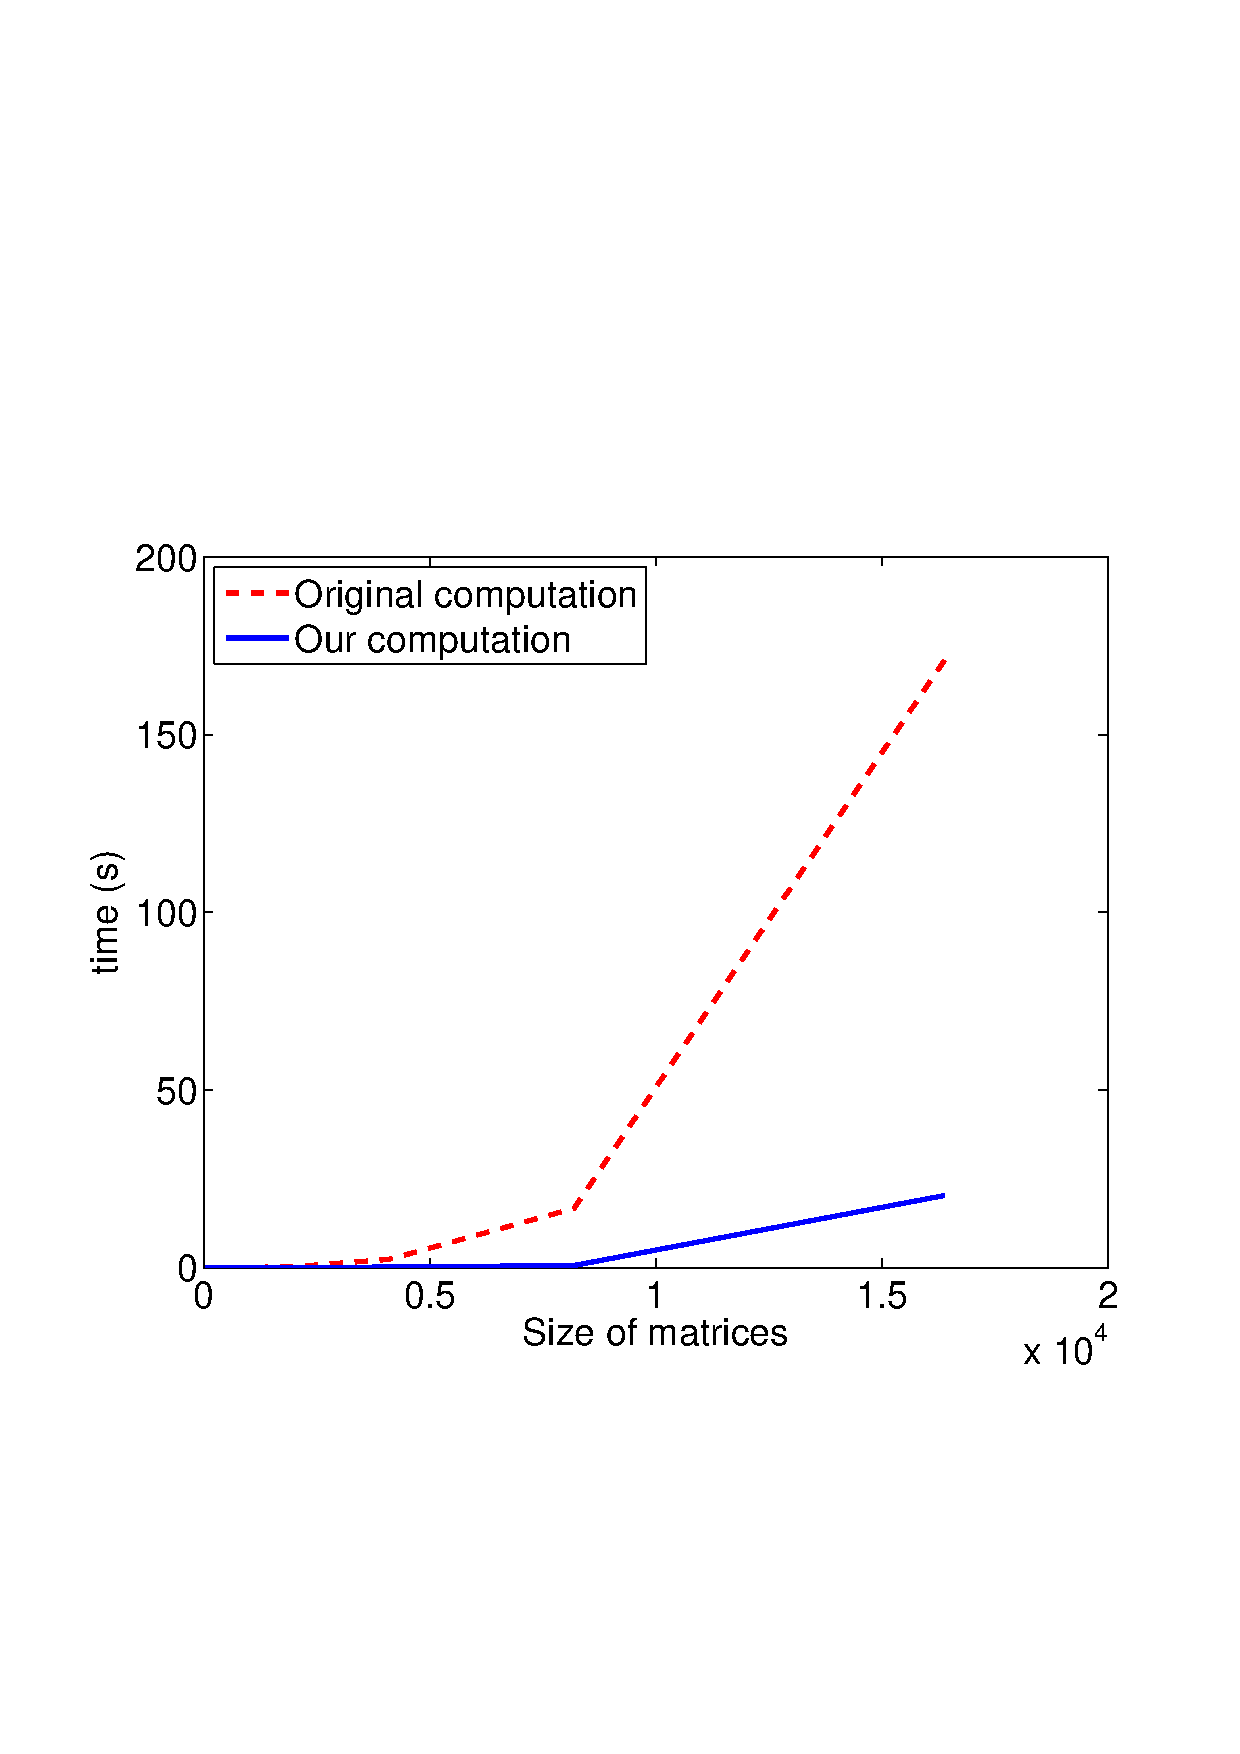
\includegraphics[scale=0.3]{img/ab.png}
\caption{Computation time for $\sum AB$ using standard algorithm vs using inferred optimal algorithm.}
\label{ab}
\end{figure}

Similarly, we found quadratic time computation, instead of cubic, for
similar expressions such as: 
\begin{align*}
	\sum ABC\text{, }\sum ABCD\text{, }\sum AA^T\text{, }\sum AA^TA
\end{align*}

As far we we are aware, these identities appear to be novel. Our
system could automatically analyze large code repositories to find
these and other expressions, which are currently computed
inefficiently. Alternativeily, our optimization rules could be placed
into compilers to generate efficient code.

\subsection{Partition Function Approximation}

As we showed in Section \ref{partitionfunction}, we can manually find
$O(n^2)$ computation of $g(x \rightarrow x^k, W)$ for $k = 1, 2$
instead of native exponential time computation. By use of our
framework, we found rules for $k = 3, 4, 5$. However for $k = 4, 5$
these rules used computation with $O(n^3)$ time (i.e.~matrix
multiplication).  Finding computational rules for higher degree
polynomials is expensive: Table \ref{grammars} shows the time
necessary to generate all the rules. It is worth noting that grammar
can be evaluated just once, and the resulting coefficients can be
stored. Furthermore, the process of discovering the computational rule
for a given power only need to be performed once. However, due to limited computational
power we analyzed only powers $k \leq 5$. As we note in Section
\ref{agenda} a future direction would be to learn patterns for
$k=2,3,4,5$ that allow us to generalize to $k>5$ without exhaustively
searching all possible rules. 

Table \ref{eval} shows number of terms necessary to derive $g(x
\rightarrow x^k, W)$ for various $k$. Figure \ref{approximations} shows
how well partition function is approximated with finite Taylor
expansion. Finally, Figure \ref{time_approx} compares computation time
of derived rules to the computation time of naive exponential time
algorithm.

\begin{table}
\tiny
\centering
\begin{tabular}{rrr}
\hline
Degree & Grammar size & Time (s) \\
\hline
2 & 5 & 17 \\
3 & 15 & 188 \\
4 & 48 & 2535\\
5 & 139 & 31320 \\
\hline
\end{tabular}
\caption{Table summarizes size and computational time for grammars of specific degree. 
All computation here are performed on expressions, and have nothing to do with computation time on instantiations.
This procedure has to be executed only once.}
\label{grammars}
\end{table}

% TODO(wojciech): \mathbf was on purpose below? it's not consistent.
% TODO(karol): we need more columns in those tables, or we should consider merging them
\begin{table}
\tiny
\centering
\begin{tabular}{rrr}
\hline
Degree & Num. terms & Complexity \\
\hline
2 & 4 & $O(n^2)$\\
3 & 5 & $O(n^2)$\\
4 & 21 & $\mathbf{O(n^3)}$\\
5 & 30 & $\mathbf{O(n^3)}$\\
\hline
\end{tabular}
\caption{Table summarizes complexity of computation of $g(x \rightarrow x^k, W)$. 
Number of terms, and complexity of every term is important for the computation of the target expression.
Potentially, we need to evaluate partition function multiple times, so the ``Complexity''
is the complexity of our final system were we use such expressions.} 
\label{eval}
\end{table}

\begin{figure}[h]
\centering
\includegraphics[scale=0.2]{img/approximations.png}
\caption{Comparison of approximations with various number of Taylor terms.}
\label{approximations}
\end{figure}



\begin{figure}[h]
\centering
\includegraphics[scale=0.24]{img/time_approx.png}
\caption{Comparison of computation time for naive exponential time algorithm vs our optimized derivation.}
\label{time_approx}
\end{figure}



\section{Dropout marginalization}
In this section we will perform analogous analisys to the one from Subsection \ref{subsubsec:gx} 
for a single layer network with $L_2$ loss. 
First, we derive update rules for weights for a single layer neural networks without any regularization. Then
we will confront it with dropout network. We will compute marginalization over
all posible dropout masks (i.e. marginalization over all masks).
We will describe how it can be discovered for
more complex networks with our framework. 


Single layer neural network with $L_2$ loss minimizes following objective:
\begin{equation*}
  \min_W ||WX - Y||^2, X \in \mathbb{R}^{f \times b}, Y \in \mathbb{R}^{g \times b}, W \in \mathbb{R}^{g \times f}
\end{equation*}
By differentiating above equation one gets gradient descent update rule
on $W$ (sign $\sim$ indicates that we drop multiplicative constants)
\begin{equation*}
 \partial W = 2(WX - Y)X^T \sim WXX^T - YX^T
\end{equation*}
We note for further derivation that $C = XX^T$ is the covariance matrix of
$X$, and that $C_{i,j} = \sum_k X_{i, k}X_{j, k}$.


Dropout minimizes following objective:
\begin{equation*}
  \argmin_W \mathbb{E}_M ||W(X .* M) - Y||^2, M \in \{0, 1\}^{f \times b}
\end{equation*}
Expectation is over all possible mask assignments, and $.*$ is 
element-wise multiplication. For simplification
let's assume that we drop neurons with probability $0.5$. Expectation
can be replaced with sum over all possible masks. Let's compute
derivative with respect to weights $W$. 
\begin{align*}
  \partial W \sim \sum_M (W(X .* M) - Y)(X .* M)^T = \\
  \sum_M W(X .* M)(X .* M)^T - Y(X .* M)^T = \\
  W\sum_M [(X .* M)(X .* M)^T] - 2^{fb - 1}YX^T= \\
\end{align*}
Let's denote $D = \sum_M (X .* M)(X .* M)^T$. 
\begin{align*}
  D_{i,j} = \sum_M \sum_k X_{i, k} X_{j, k} M_{i, k} M_{j, k} \\
  D_{i,j} \text{ for } i \neq j = 2^{fg - 2} \sum_k X_{i, k} X_{j, k} = 2^{fg - 2}C_{i, j} \\
  D_{i,j} \text{ for } i = j = 2^{fg - 1} \sum_k X_{i, k} X_{j, k} = 2^{fg - 1}C_{i, j} \\
  D = 2^{fg - 2}(XX^T + XX^T .* I) \text { $I$ is identity matrix } \\
  \partial W \sim \frac{1}{2}W (XX^T + XX^T .* I) - YX^T
\end{align*}

Above derivation of dropout marginalization can be discovered by our framework, and can be generalized
to multiple layer network with rational (quotient of two polynomials) activation functions. 
More formally, it means that framework is able to discover how to update weights $W$ for the following
objective:
\begin{equation*}
  \argmin_{W_1, W_2} \mathbb{E}_{M_1, M_2} ||W_2(f(W_1(X .* M_1)) .* M_2) - Y||^2
\end{equation*}
$f$ in this equation is a rational function.


\section{Data augmentation marginalization}

\section{Discussion and Future Work}

We have presented an automatic method for discovery of computations for
 polynomial expressions. The method itself is novel, as well as the derived
approximations to the RBM partition function.  There are four
major directions of future research. 


The first is focus on extension of our method
to (i) reacher class of functions than polynomials, (ii) larger set of production
rules, (iii) more complex objects than matrices (e.g. tensors).


The second would be to use learning to
generalize computation (Subsection \label{agenda)}, i.e.~replace current brute force process with
something more intelligent. E.g. We could generalize computation of
$g(x \rightarrow x^k, W)$ for $k = 1, \dots, 5$ to $k > 5$. 


The third is concerned with computing
the partition function and its derivatives, using approximations for
learning, approximations for deep Bolzmann machines, optimization of
the derived formulas, and understanding the mathematical principles behind
formulas derived by our programs. 


Finally,
the forth direction are real-world applictions of this framework on
large code databases. We could automatically detect parts of code with
expressions that have suboptimal time complexity and replace them.


We discuss in following subsections two first major directions of future research.


\subsection{Extension of Grammar}
The presented framework has some limitations, but also can be easily extended. First,
we operate on polynomials instead of general functions. It is quite easy to verify
equality of polynomials, because it is enough to check equality of coefficients or
evaluations on sufficiently many points (more than degree of
polynomial). However, for generic functions
it is not as simple. For example, if our basis would to include trigonometric functions, then the
framework would have to be aware of many additional identities,
e.g. $\sin^2{x} + \cos^2{x} = 1$, or $2\sin x \cos x = \sin
2x$. Although challenging, we believe it is possible to extend our
framework to handle such cases. 

It is straight forward to extend our framework to matrices of fractional
polynomials instead of matrices of polynomials.  We could
then include productions like matrix inverse and element-wise inverse of
a matrix.  Another direction would be to generlize matrices to arbitrary tensors
for which it is even harder for humans to spot useful relations.

Finally, we are interested in exploiting productions which could discover 
recurrences. This would allow the discovery the fast fourier ransform, or
Strassen's algorithm for fast matrix multiplication. This family of problems is quite broad,
and crucial in computation.


\subsection{Computation Generalization}\label{agenda}

This paper presents a brute force search over all possible computations, 
to yield terms that could lead to the target result. Although it works
well for polynomials of small degrees $k \leq 5$, for larger powers 
brute force methods seems to fail. One of the contributions of this paper is to
demonstrate how a small subset of mathematics may be explored with an automatic proving
system. However, to broaden the range of math that we can address, we
must move beyond brute force methods to more intelligent approaches
which learn which rules are likely to be helpful, based on expressions
for smaller powers. This would allow us move to polynomials of $k>5$,
making accurate estimation of the partition function for many deep
networks possible. More broadly, it would bring machine learning techniques
to the area of automatic theorem proving, which is another domain of
human intelligence distinct from perceptual tasks (where machine
learning is already effective). 

%  tackle a broader set of problems We look forward to extend this brute force methods to more intelligible approaches, which
% could learn based on rules for smaller powers, how to solve problem for larger powers. This would
% have two-fold implications in machine learning. Firstly, it would bring machine learning techniques
% to the area of automatic theorem proving, which another domain of human intelligence after perception
% of vision, or hearing. Secondly, solution to the problem of partition function approximation
% could have consequences in unsupervised learning of RBMs, deep Bolzmann machines, and deep
% belief networks. 






\nocite{*}
\bibliography{bibliography}
\bibliographystyle{abbrvnat}

\end{document} 

